\documentclass{standalone}
\usepackage{tikz}
\usetikzlibrary{positioning}
\usetikzlibrary {shapes.geometric}
\usepackage[nomessages]{fp}

% We will update these variables to reuse commands within a diagram
\newcommand{\checkpointRow}{Checkpoints}
\newcommand{\rollupRow}{L2}
\newcommand{\col}{black}

\tikzstyle{blob} = [draw, rectangle, minimum width=0.5cm, minimum height=0.5cm, anchor=west, inner sep=0, outer sep=0]
\tikzstyle{segment} = [fill, rectangle, minimum height=0.5cm, anchor=west, color=\col, inner sep=0, outer sep=0]
\tikzstyle{pubHash} = [draw, circle, color=\col, anchor=west]
\tikzstyle{block} = [draw, rectangle, color=\col, minimum width=0.1cm, minimum height=0.5cm, anchor=west]
\tikzstyle{checkpoint} = [fill, diamond,color=\col, inner sep=2, anchor=west]
\tikzstyle{txOrigin} = [circle, draw, fill=lightgray, inner sep=2]
\tikzstyle{contract} = [rectangle, rounded corners, text centered, draw, inner sep=10pt]
\tikzstyle{arrow} = [->]

\newcommand{\timeline}{
    \node (t0) at (0,0) {};
    \node (tEnd) at (13,0) {};
    \node (genesis) at (1.5, 0) {};
    \node (start) at (2, 0) {};
    \node (origin) at (t0) [xshift=-0.7cm] {};
    \draw (origin) [->, thick]  -- (tEnd);
}

\newcommand{\structure}{
    \timeline
    \node (PubHashes) [gray, above of=t0] {Pub Hashes};
    \node (lastPubHash) at (genesis |- PubHashes) [pubHash] {};
    \node (Blobs) [gray, above of=PubHashes] {Blobs};
    \node (L1) [above of=Blobs] {L1};

    \node (nextBlob) at (start |- Blobs) {};
    \node (nextPubHash) at (nextBlob |- PubHashes) {};
}

% Usage: blobs{X} where X is the number of blobs in a group
\newcommand{\blobs}[1]{
    \foreach \blobIdx in {1,...,#1}{
        \node (nextBlob) [blob] at (nextBlob.east) {};
    };
    % create space after blob group
    \node (nextBlob) [right=of nextBlob.east] {};
    \node (nextPubHash) at (nextBlob |- PubHashes) {};
}

\newcommand{\pubHash} {
    \node (arrowStart) at (nextPubHash) [xshift=0.1cm] {};
    \draw [arrow] (arrowStart) -- (lastPubHash);
    \node (lastPubHash) [pubHash] at (nextPubHash) {};
    \node (nextPubHash) at (lastPubHash) [xshift=0.3cm] {};
}

\begin{document}

% Introduce Publication Feed
\ifnum \sourceNo = 0
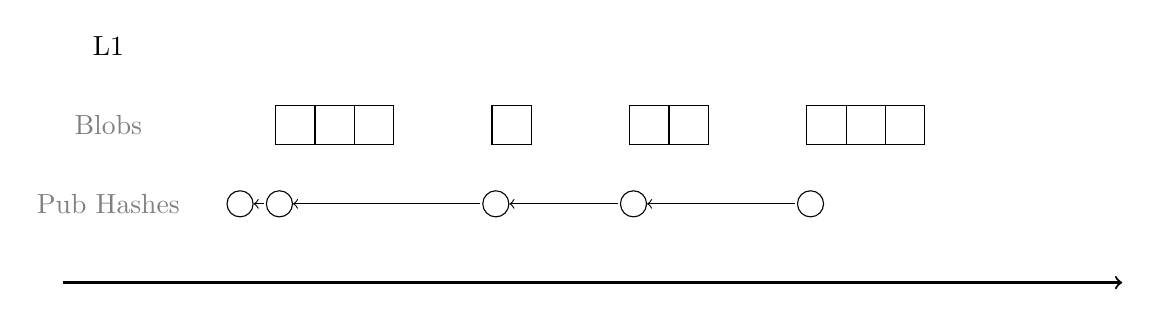
\begin{tikzpicture}
    \structure
    \pubHash \blobs{3} 
    \pubHash \blobs{1}
    \pubHash \blobs{2}
    \pubHash \blobs{3}
\end{tikzpicture}
\fi

% Introduce Rollup Inbox
\ifnum \sourceNo = 1
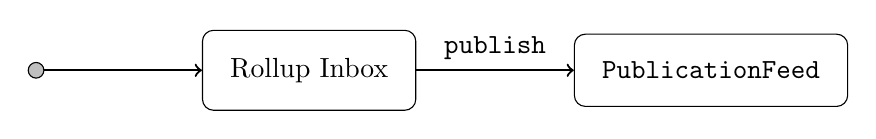
\begin{tikzpicture}[node distance=2cm]
    \node (origin) at (0,0) [txOrigin] {};
    \node (inbox) [right=of origin, contract] {Rollup Inbox};
    \node (pubFeed) [right=of inbox, contract] {\texttt{PublicationFeed}};
    \draw [->, thick] (origin) -- (inbox);
    \draw [->, thick] (inbox) -- node[anchor=south] {\texttt{publish}} (pubFeed) ;
\end{tikzpicture}
\fi

% Hack: just overwrite the timeline structure as new features are introduced
% This should be refactored to avoid duplication
% In this case, add the L2 row
\renewcommand{\structure}{
    \timeline
    \node (PubHashes) [gray, above of=t0] {Pub Hashes};
    \node (lastPubHash) at (genesis |- PubHashes) [pubHash] {};
    \node (Blobs) [gray, above of=PubHashes] {Blobs};
    \node (L1) [above of=Blobs] {L1};
    \node (L2) [below of=t0] {L2};

    \node (nextBlob) at (start |- Blobs) {};
    \node (nextPubHash) at (nextBlob |- PubHashes) {};
}

% Usage: \rollupBlocks{count}
\newcommand{\rollupBlocks}[1]{
    \node (lastBlock) at (lastPubHash |- \rollupRow) {};
    \foreach \block in {1,...,#1}{
        \node (lastBlock) [block] at (lastBlock.east) {};
    };
}

% Introduce L2 blocks
\ifnum \sourceNo = 2
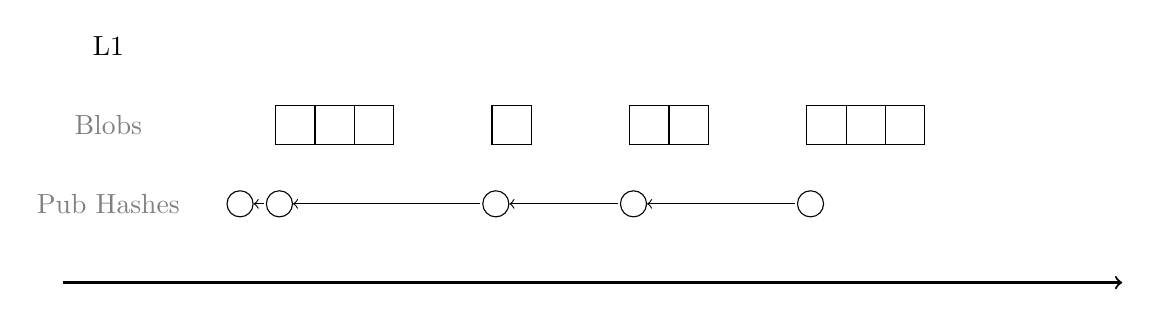
\begin{tikzpicture}
    \structure
    \pubHash \blobs{3} \rollupBlocks{8}
    \pubHash \blobs{1} \rollupBlocks{5}
    \pubHash \blobs{2} \rollupBlocks{7}
    \pubHash \blobs{3} \rollupBlocks{10}
\end{tikzpicture}
\fi

% Hack: just overwrite the timeline structure as new features are introduced
% This should be refactored to avoid duplication
% In this case, add a Checkpoints row
\renewcommand{\structure}{
    \timeline
    \node (Checkpoints) [gray, above of=t0] {Checkpoints} {};
    \node (PubHashes) [gray, above of=Checkpoints] {Pub Hashes};
    \node (lastPubHash) at (genesis |- PubHashes) [pubHash] {};
    \node (Blobs) [gray, above of=PubHashes] {Blobs};
    \node (L1) [above of=Blobs] {L1};
    \node (L2) [below of=t0] {L2};

    \node (nextBlob) at (start |- Blobs) {};
    \node (nextPubHash) at (nextBlob |- PubHashes) {};
}

% Usage: \rollupBlocks{count}
% Add a checkpoint after all blocks
\renewcommand{\rollupBlocks}[1]{
    \node (lastBlock) at (lastPubHash |- \rollupRow) {};
    \foreach \block in {1,...,#1}{
        \node (lastBlock) [block] at (lastBlock.east) {};
    };
    \node (lastCheckpoint) [checkpoint] at (lastBlock.east) {};
}

\newcommand{\saveCheckpoint}{
    \node (savedCheckpoint) [checkpoint] at (lastCheckpoint.west |- \checkpointRow) {};
}

\newcommand{\genesisCheckpoint} {
    \node (lastCheckpoint) [checkpoint] at (genesis |- \rollupRow) {};
}

% Introduce Checkpoints
\ifnum \sourceNo = 3
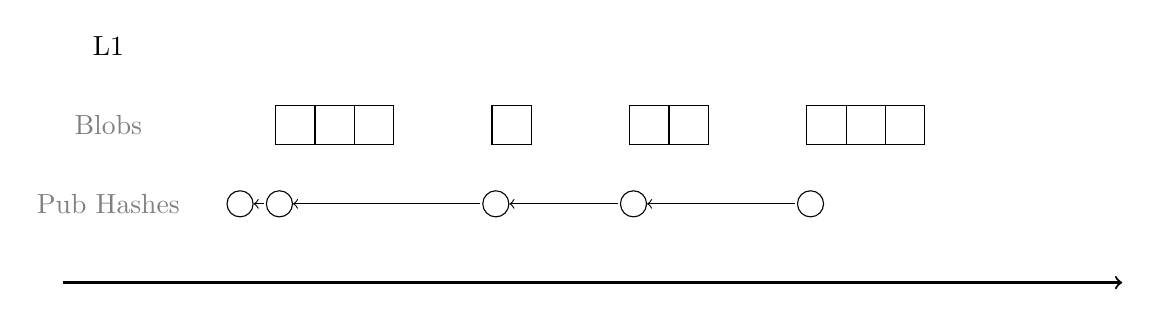
\begin{tikzpicture}
    \structure
    \genesisCheckpoint \saveCheckpoint

    \pubHash \blobs{3} \rollupBlocks{8} \saveCheckpoint
    \pubHash \blobs{1} \rollupBlocks{5}
    \pubHash \blobs{2} \rollupBlocks{7}
    \pubHash \blobs{3} \rollupBlocks{10} \saveCheckpoint
\end{tikzpicture}
\fi


% Hack: just overwrite the timeline structure as new features are introduced
% This should be refactored to avoid duplication
% In this case, split the Checkpoints and L2 rows to accomodate two rollups
\renewcommand{\structure}{
    \timeline
    \node (CheckpointsB) [gray, above of=t0] {Checkpoints B} {};
    \node (CheckpointsA) [gray, above of=CheckpointsB] {Checkpoints A} {};
    \node (PubHashes) [gray, above of=CheckpointsA] {Pub Hashes};
    \node (lastPubHash) at (genesis |- PubHashes) [pubHash] {};
    \node (Blobs) [gray, above of=PubHashes] {Blobs};
    \node (L1) [above of=Blobs] {L1};
    \node (RollupA) [below of=t0] {Rollup A};
    \node (RollupB) [below of=RollupA] {Rollup B};

    \node (nextBlob) at (start |- Blobs) {};
    \node (nextPubHash) at (nextBlob |- PubHashes) {};
}

\newcommand{\switchToA}{
    \renewcommand{\checkpointRow}{CheckpointsA}
    \renewcommand{\rollupRow}{RollupA}
    \renewcommand{\col}{blue!30}
}

\newcommand{\switchToB}{
    \renewcommand{\checkpointRow}{CheckpointsB}
    \renewcommand{\rollupRow}{RollupB}
    \renewcommand{\col}{red!30}
}

% Usage: blobs{X}{sizeA} where 
%   X is the number of blobs in a group
%   sizeA is the number of blobs the first rollup segment occupies (the second segment is whatever is left)
\renewcommand{\blobs}[2]{
    \FPeval{\sizeB}{#1 - #2}  

    \switchToA
    \node (nextSegment) at (nextBlob.east) [segment, minimum width=#2 * 0.5cm] {};
    \switchToB
    \node (nextSegment) at (nextSegment.east) [segment, minimum width=\sizeB * 0.5cm] {};

    \foreach \blobIdx in {1,...,#1}{
        \node (nextBlob) [blob] at (nextBlob.east) {};
    };
    % create space after blob group
    \node (nextBlob) [right=of nextBlob.east] {};
    \node (nextPubHash) at (nextBlob |- PubHashes) {};
}


% Shared Blobs
\ifnum \sourceNo = 4
% Suppress the pub hashes row for now
% We still create invisible elements so they can be used to position the other elements
\tikzstyle{pubHash} = [circle, color=\col, anchor=west] % remove "draw"
\tikzstyle{arrow} = [opacity=0]

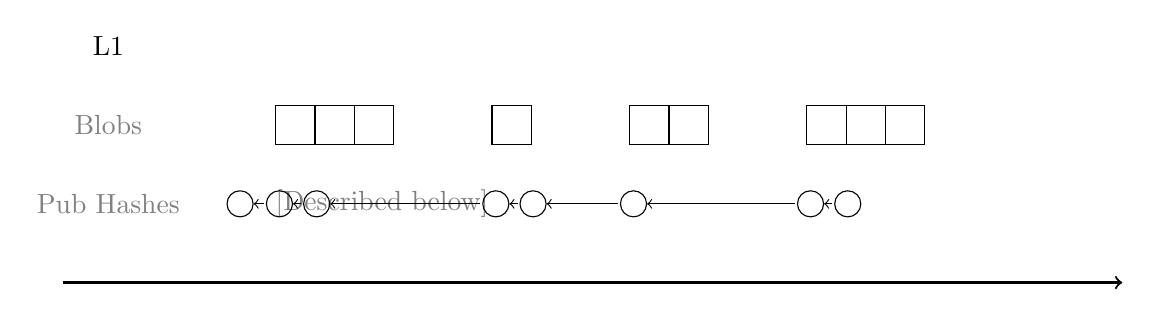
\begin{tikzpicture}
    \structure
    \node [gray, anchor=west] at (nextPubHash) {[Described below]};

    \switchToA \genesisCheckpoint \saveCheckpoint
    \switchToB \genesisCheckpoint \saveCheckpoint

    \switchToA \pubHash \rollupBlocks{5}
    \switchToB \pubHash \rollupBlocks{6} \saveCheckpoint
    \blobs{3}{1.3}

    \switchToA \pubHash \rollupBlocks{5}
    \switchToB \pubHash \rollupBlocks{2}
    \blobs{1}{0.6}

    \switchToB \pubHash \rollupBlocks{5} 
    \blobs{2}{0}
    
    \switchToA \pubHash \rollupBlocks{8} \saveCheckpoint
    \switchToB \pubHash \rollupBlocks{3} \saveCheckpoint
    \blobs{3}{1.8}
\end{tikzpicture}
\fi

% Hack: just overwrite the timeline structure as new features are introduced
% This should be refactored to avoid duplication
% In this case, rename Rollup A to Taiko (the variables still use A for simplicity)
% Also denote the `lastPubHash' as the `lastTaikoPubHash` as well
\renewcommand{\structure}{
    \timeline
    \node (CheckpointsB) [gray, above of=t0] {Checkpoints B} {};
    \node (CheckpointsA) [gray, above of=CheckpointsB] {Checkpoints Taiko} {};
    \node (PubHashes) [gray, above of=CheckpointsA] {Pub Hashes};
    \node (lastPubHash) at (genesis |- PubHashes) [pubHash] {};
    \node (Blobs) [gray, above of=PubHashes] {Blobs};
    \node (L1) [above of=Blobs] {L1};
    \node (RollupA) [below of=t0] {Taiko};
    \node (RollupB) [below of=RollupA] {Rollup B};

    \node (nextBlob) at (start |- Blobs) {};
    \node (nextPubHash) at (nextBlob |- PubHashes) {};
    \node (lastTaikoPubHash) at (lastPubHash) {};
}

\newcommand{\taikoPubHash} {
    \pubHash
    \draw [arrow, color=\col] (lastPubHash) to[bend left] (lastTaikoPubHash); 
    \node (lastTaikoPubHash) at (lastPubHash) {};
}

% Non-shared publications
\ifnum \sourceNo = 5
\begin{tikzpicture}
    \structure

    \switchToA \genesisCheckpoint \saveCheckpoint
    \switchToB \genesisCheckpoint \saveCheckpoint

    \switchToA \taikoPubHash \rollupBlocks{5}
    \switchToB \pubHash \rollupBlocks{6} \saveCheckpoint
    \blobs{3}{1.3}

    \switchToA \taikoPubHash \rollupBlocks{5}
    \switchToB \pubHash \rollupBlocks{2}
    \blobs{1}{0.6}

    \switchToB \pubHash \rollupBlocks{5} 
    \blobs{2}{0}
    
    \switchToA \taikoPubHash \rollupBlocks{8} \saveCheckpoint
    \switchToB \pubHash \rollupBlocks{3} \saveCheckpoint
    \blobs{3}{1.8}
\end{tikzpicture}
\fi


\end{document}



        